% !TEX root = ../main.tex
\paragraph{Tracking}
    Charged particle tracking is the key element of the CLAS12 event reconstruction.
    It is separated into the reconstruction of tracks in the central tracker system and the forward tracking system.

    In the forward region, the torus magnet bends charged particles inward toward the beamline or outward of it depending on their charge.
    At full nominal current, the $\int Bdl$ varies from $2 \text{Tm}$ at $5\degree$ to $0.5 \text{Tm}$ at $40\degree$.
    The forward tracking system in charge of tracking in this region is comprised of the Forward MicroMegas Tracker (FMT) and the Drift Chambers (DC).

    In the central region, the $5 \text{T}$ solenoidal magnetic field bends charged tracks into helices.
    In it, the central tracking system is comprised of the Silicon Vertex Tracker (SVT) and the Barrel MicroMegas Tracker (BMT), which together form the Central Vertex Tracker (CVT).

% --+ Reconstruction +----------------------------------------------------------
    \begin{wrapfigure}{l}{0.50\textwidth}
        \centering\frame{
        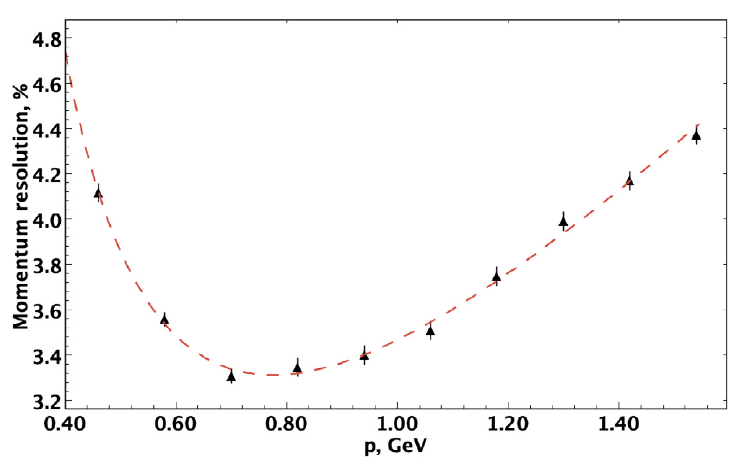
\includegraphics[width=\linewidth]{11experiment/img/23cvt_pres.png}}
        \caption[CVT momentum resolution vs. momentum.]{Momentum resolution vs. momentum of simulated protons in the CVT without background.}
        \label{fig::cvt_pres}
    \end{wrapfigure}

    For both systems, track reconstruction comprises algorithms for pattern recognition and track fitting. Hit objects, corresponding to the passage of a particle through a particular detector component, require the transformation of an electronic signal into a location of the track’s
    position in the detector subsystem geometry.
    A hit is defined as a detector element represented by a geometric object, for example, a line representing a strip in the central tracker.
    These objects then form the input to the pattern recognition algorithms.

    \begin{figure}[t]
        \centering\frame{
        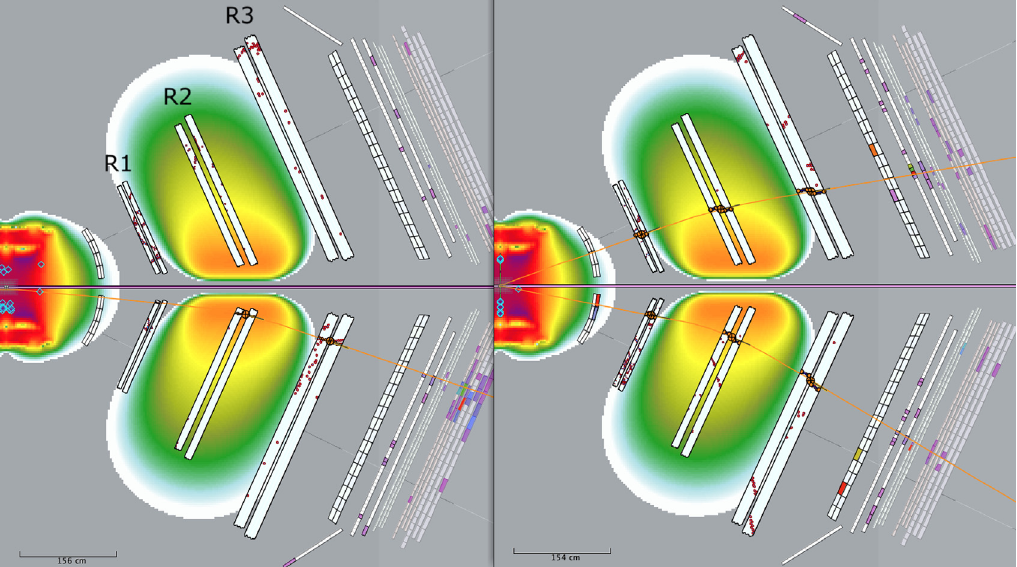
\includegraphics[width=\textwidth]{11experiment/img/23ced_event.png}}
        \caption[Particle going through DC.]{Views from CLAS12 Event Display (ced) of charged particle tracks in the DC showing cut-views to highlight different pairs of sectors of the CLAS12 Forward Detector.
        The coloured detector elements are the registered hits and the orange lines are the result of track reconstruction using the hits in the DC.
        The coloured areas about the detectors represent the regions of magnetic field from the torus and the solenoid.
        In these views the beam is incident from the left and the target is located in the middle of the solenoid (at the left edge of the image).}
        \label{fig::ced_event}
    \end{figure}

    Pattern recognition involves the identification of clusters of hits and the determination of the spatial coordinates and corresponding uncertainties for the hits and clusters.
    At the pattern recognition stage, hits that are consistent with belonging to a trajectory (such as a particle track) are identified.
    This set of hits is then fit to the expected trajectory with their uncertainties, incorporating the knowledge of the detector material and the detailed magnetic field map.
    An illustration of a particle going through the DC can be seen in Figure \ref{fig::ced_event}.

% --+ Performance +-------------------------------------------------------------
    The momentum resolutions in the central and forward trackers as a function of momentum are shown in Figures \ref{fig::cvt_pres} and \ref{fig::dc_pres} respectively.
    The distributions are fit with a function of the form $\sqrt{a + bx^2 + c/(1 + d/x^2)}$.
    In both distributions, the worsening of the resolution at low momentum is due to multiple scattering effects.
    The resolution also worsens as a function of momentum after a minimum is reached due to poorer track curvature resolution.

    \begin{wrapfigure}{r}{0.50\textwidth}
        \centering\frame{
        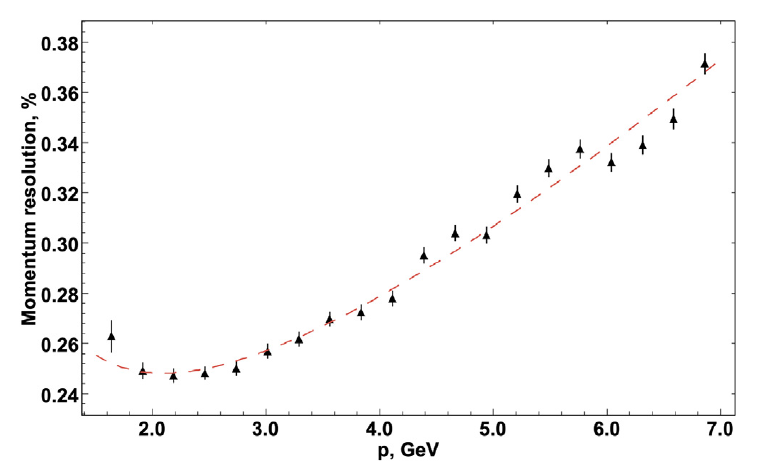
\includegraphics[width=\linewidth]{11experiment/img/23dc_pres.png}}
        \caption[DC momentum resolution vs momentum.]{Momentum resolution vs. momentum in the DC evaluated using pions simulated at $\theta = 15\degree \pm 5\degree$ and at $\phi = 0 \pm 5\degree$ without background.}
        \label{fig::dc_pres}
    \end{wrapfigure}

    For central tracking, an average CVT reconstruction efficiency of $87.3\%$ is obtained from a simulated proton sample with momenta in the range from $0.5$ to $2.5 \text{GeV}$.
    A slight drop of efficiency is observed for tracks with momenta less than $600 \text{MeV}$.
    The higher curvature of small $\text{p}_\perp$ tracks results in an increase in inefficiency due to acceptance effects.
    The dominant source of inefficiency is the gaps between the sensitive volumes for the BMT and the SVT.

    For forward tracking, the momentum resolution in the DC is evaluated using tracks simulated at $\theta = 15\degree \pm 5\degree$ and at $\phi = 0 \pm 5\degree$.
    This is to ensure that most tracks are within the sensitive volume.
    Furthermore, the DC momentum resolution is correlated with the polar angle since the track curvature is determined from the magnetic field intensity, which is higher at lower angles in the torus field.
    These resolutions are obtained from a Monte Carlo sample that does not include out-of-time backgrounds or misalignments of the tracking volumes \cite{ziegler2020}.
